% 基礎数学 第10回 ベクトルの基礎（CC BY-SA 4.0）
\documentclass[aspectratio=169]{beamer}
\usepackage{lfs-slides}
\lfscourse{基礎数学}

\title{ベクトルの基礎}
\subtitle{基礎数学 第10回}
\author{}
\date{}

\begin{document}

\begin{frame}
  \titlepage
\end{frame}

\begin{frame}{今日のねらい}
  \lfsmessage{ベクトル ＝ 向きと大きさをもつ量}
  \bigskip
  \begin{itemize}
    \item ベクトルの表し方と、等しいベクトル
    \item 和・差・スカラー倍（図と成分の両方で）
    \item 寄り道と基準点で式を変形する
    \item 内分点・重心
    \item 工学では：力の合成
  \end{itemize}
\end{frame}

\section{ベクトルとは}

\begin{frame}{スカラーとベクトル}
  \begin{columns}[t]
    \column{0.5\textwidth}
      \begin{block}{スカラー：大きさだけ}
        質量 $3$ kg，\ 温度 $20^\circ$C，\ 時間 $5$ 秒
      \end{block}
    \column{0.5\textwidth}
      \begin{block}{ベクトル：向きと大きさ}
        速度（北へ時速 $40$ km），\ 力（右へ $10$ N）
      \end{block}
  \end{columns}
  \bigskip
  \begin{center}
    \begin{tikzpicture}[>=stealth]
      \fill (0,0) circle (2pt) node[below left] {A};
      \fill (4,1.2) circle (2pt) node[above right] {B};
      \draw[->,very thick,blue] (0,0) -- (4,1.2);
      \node[blue,above] at (1.7,1.0) {$\overrightarrow{\mathrm{AB}}$ \ または \ $\vec{a}$};
    \end{tikzpicture}
  \end{center}
  矢印の長さが大きさ：$|\vec{a}|$ と書く
\end{frame}

\begin{frame}{等しいベクトル}
  \lfsmessage{向きと大きさが同じなら、場所が違っても同じベクトル}
  \begin{center}
    \begin{tikzpicture}[>=stealth]
      \foreach \x/\y in {0/0, 3/1.2, 6.5/-0.3, 1.5/-1.4}
        \draw[->,very thick,blue] (\x,\y) -- ++(2,0.8);
      \node[blue] at (9.6,0.3) {すべて $\vec{a}$};
    \end{tikzpicture}
  \end{center}
  {\small 矢印は「平行移動しても同じもの」とみなす}
\end{frame}

\section{和・差・スカラー倍}

\begin{frame}{和：矢印をつなぐ}
  \begin{columns}[c]
    \column{0.5\textwidth}
      \begin{center}
        % ベクトルの和：つなぐ（三角形）と平行四辺形
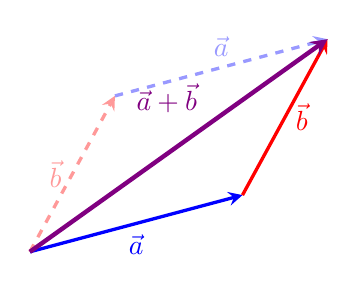
\begin{tikzpicture}[scale=0.9,>=stealth]
  \coordinate (O) at (0,0);
  \coordinate (A) at (3,0.8);
  \coordinate (C) at (4.2,3);
  \coordinate (B) at (1.2,2.2);
  \draw[->,very thick,blue] (O) -- (A) node[midway,below] {$\vec{a}$};
  \draw[->,very thick,red] (A) -- (C) node[midway,right] {$\vec{b}$};
  \draw[->,very thick,red!40,dashed] (O) -- (B) node[midway,left] {$\vec{b}$};
  \draw[->,very thick,blue!40,dashed] (B) -- (C) node[midway,above] {$\vec{a}$};
  \draw[->,ultra thick,violet] (O) -- (C) node[pos=0.6,above left] {$\vec{a}+\vec{b}$};
\end{tikzpicture}

      \end{center}
    \column{0.5\textwidth}
      \begin{itemize}
        \item $\vec{a}$ の終点から $\vec{b}$ をかく → 始点から終点へ
        \item 平行四辺形の対角線と同じ
        \item 順番を変えても同じ：$\vec{a} + \vec{b} = \vec{b} + \vec{a}$
      \end{itemize}
  \end{columns}
\end{frame}

\begin{frame}{スカラー倍と差}
  \begin{center}
    % スカラー倍・逆ベクトル
\begin{tikzpicture}[scale=0.85,>=stealth]
  \draw[->,very thick,blue] (0,0) -- (1.5,0.75) node[above] {$\vec{a}$};
  \draw[->,very thick,blue!70!black] (2.5,0) -- (5.5,1.5) node[above] {$2\vec{a}$};
  \draw[->,very thick,red] (8,0.75) -- (6.5,0) node[below] {$-\vec{a}$};
\end{tikzpicture}

  \end{center}
  \begin{itemize}
    \item $k\vec{a}$：向きはそのまま（$k<0$ なら逆向き）、長さ $|k|$ 倍
    \item $-\vec{a}$：同じ長さで逆向き
    \item 差は「逆向きを足す」：$\vec{a} - \vec{b} = \vec{a} + (-\vec{b})$
  \end{itemize}
\end{frame}

\begin{frame}{成分で計算する}
  \lfsmessage{成分ごとに足す・かける}
  \[
    \vec{a} = (a_1,\, a_2),\quad \vec{b} = (b_1,\, b_2)
  \]
  \begin{align*}
    \vec{a} + \vec{b} &= (a_1 + b_1,\ a_2 + b_2) &
    k\vec{a} &= (k a_1,\ k a_2) &
    |\vec{a}| &= \sqrt{a_1^2 + a_2^2}
  \end{align*}
  \medskip
  例：$\vec{a} = (3,\, 4)$，$\vec{b} = (1,\, -2)$ のとき
  \[
    \vec{a} + \vec{b} = (4,\, 2), \qquad 2\vec{a} - \vec{b} = (5,\, 10), \qquad |\vec{a}| = \sqrt{9 + 16} = 5
  \]
\end{frame}

\section{式の変形}

\begin{frame}{寄り道と基準点}
  \begin{columns}[t]
    \column{0.5\textwidth}
      \begin{block}{寄り道：途中の点をはさむ}
        \[
          \overrightarrow{\mathrm{AB}} = \overrightarrow{\mathrm{AP}} + \overrightarrow{\mathrm{PB}}
        \]
        {\small A → P → B と回り道しても、行き先は同じ}
      \end{block}
    \column{0.5\textwidth}
      \begin{block}{基準点：O から見る}
        \[
          \overrightarrow{\mathrm{AB}} = \overrightarrow{\mathrm{OB}} - \overrightarrow{\mathrm{OA}}
        \]
        {\small 「終点 − 始点」と覚える}
      \end{block}
  \end{columns}
  \medskip
  例：$\overrightarrow{\mathrm{AB}} + \overrightarrow{\mathrm{BC}} + \overrightarrow{\mathrm{CD}} = \overrightarrow{\mathrm{AD}}$
  \medskip

  例：A$(1,\,2)$，B$(4,\,6)$ のとき \ $\overrightarrow{\mathrm{AB}} = (4-1,\ 6-2) = (3,\, 4)$
\end{frame}

\section{内分点と重心}

\begin{frame}{内分点}
  \begin{columns}[c]
    \column{0.45\textwidth}
      \begin{center}
        % 線分 AB を m:n に内分する点 P（図は 2:1）
\begin{tikzpicture}[scale=1.0,>=stealth]
  \coordinate (O) at (0,0);
  \coordinate (A) at (0.5,2.6);
  \coordinate (B) at (4.5,1.4);
  \coordinate (P) at ($(A)!2/3!(B)$);
  \draw[thick] (A) -- (B);
  \draw[->,thick,blue] (O) -- (A) node[midway,left] {$\vec{a}$};
  \draw[->,thick,blue] (O) -- (B) node[midway,below] {$\vec{b}$};
  \draw[->,very thick,violet] (O) -- (P) node[pos=0.55,above] {$\vec{p}$};
  \fill (A) circle (2pt) node[above] {A};
  \fill (B) circle (2pt) node[right] {B};
  \fill (P) circle (2pt) node[above right] {P};
  \fill (O) circle (2pt) node[below left] {O};
  \node[above,font=\small] at ($(A)!0.33!(B)$) {$m$};
  \node[above,font=\small] at ($(A)!0.84!(B)$) {$n$};
\end{tikzpicture}

      \end{center}
    \column{0.55\textwidth}
      線分 AB を $m:n$ に内分する点 P
      \[
        \vec{p} = \frac{n\,\vec{a} + m\,\vec{b}}{m + n}
      \]
      {\small 遠い方の点に、近い方の比をかける}
      \medskip

      中点（$1:1$）：$\vec{p} = \dfrac{\vec{a} + \vec{b}}{2}$
  \end{columns}
\end{frame}

\begin{frame}{重心}
  \lfsmessage{三角形の重心 ＝ 3つの頂点の平均}
  \[
    \vec{g} = \frac{\vec{a} + \vec{b} + \vec{c}}{3}
  \]
  例：A$(0,\,0)$，B$(6,\,0)$，C$(3,\,6)$ の重心は
  \[
    \left(\frac{0 + 6 + 3}{3},\ \frac{0 + 0 + 6}{3}\right) = (3,\, 2)
  \]
\end{frame}

\section{工学では}

\begin{frame}{力の合成}
  \begin{columns}[c]
    \column{0.45\textwidth}
      \begin{center}
        % 力の合成：F1 = (3, 0)、F2 = (0, 4) → 合力 (3, 4)
\begin{tikzpicture}[scale=0.6,>=stealth]
  \draw[->] (-0.5,0) -- (4.5,0) node[right] {$x$};
  \draw[->] (0,-0.5) -- (0,5) node[above] {$y$};
  \fill[gray!50] (-0.3,-0.3) rectangle (0.3,0.3);
  \draw[->,very thick,blue] (0,0) -- (3,0) node[below] {$\vec{F}_1 = (3,\,0)$};
  \draw[->,very thick,red] (0,0) -- (0,4) node[left] {$\vec{F}_2 = (0,\,4)$};
  \draw[dashed] (3,0) -- (3,4) -- (0,4);
  \draw[->,ultra thick,violet] (0,0) -- (3,4) node[above right] {合力 $(3,\,4)$};
\end{tikzpicture}

      \end{center}
    \column{0.55\textwidth}
      2つの力が同時にはたらくと、\\
      \textbf{ベクトルの和}の力が1つはたらくのと同じ
      \[
        (3,\, 0) + (0,\, 4) = (3,\, 4)
      \]
      大きさは $\sqrt{9 + 16} = 5$ N
      \medskip

      {\small 橋・建物の設計、ロボットや車両の運動の計算で使う}
  \end{columns}
\end{frame}

\begin{frame}{まとめ}
  \begin{itemize}
    \item ベクトル：向きと大きさ。平行移動しても同じ
    \item 和はつなぐ、差は逆向きを足す、$k$ 倍は長さを $|k|$ 倍
    \item 成分で計算：成分ごと、大きさは $\sqrt{a_1^2 + a_2^2}$
    \item 寄り道 $\overrightarrow{\mathrm{AB}} = \overrightarrow{\mathrm{AP}} + \overrightarrow{\mathrm{PB}}$，\
          基準点 $\overrightarrow{\mathrm{AB}} = \overrightarrow{\mathrm{OB}} - \overrightarrow{\mathrm{OA}}$
    \item 内分点 $\dfrac{n\vec{a} + m\vec{b}}{m + n}$，\ 重心 $\dfrac{\vec{a} + \vec{b} + \vec{c}}{3}$
  \end{itemize}
  \bigskip
  \lfsmessage{次回：行列の基礎}
\end{frame}

\end{document}
